\documentclass[10pt,a4paper,twocolumn]{article}

\usepackage[colorinlistoftodos]{todonotes}
\usepackage[affil-it]{authblk}
\usepackage{titlesec}
\usepackage{enumitem}

\usepackage{url}
\urldef{\mailsa}\path|{i.c.t.m.speek}@student.tudelft.nl|
\newcommand{\keywords}[1]{\par\addvspace\baselineskip%
\noindent\keywordname\enspace\ignorespaces#1}

\titlespacing\section{0pt}{20pt plus 4pt minus 2pt}{8pt plus 2pt minus 2pt}
\titlespacing\subsection{0pt}{12pt plus 4pt minus 2pt}{5pt plus 2pt minus 2pt}
\titlespacing\subsubsection{0pt}{12pt plus 4pt minus 2pt}{5pt plus 2pt minus 2pt}

% first the title is needed
\title{ScavengeIT - a face verification based photo database scavenger}


\author{I.C.T.M Speek%
		\thanks{Electronic address: \texttt{i.c.t.m.speek@student.tudelft.nl}; Corresponding author}}
\affil{Computer Vision \\ Delft University of Technology}

% the affiliations are given next; don't give your e-mail address
% unless you accept that it will be published

\begin{document}

\maketitle

%------------------------------------------------------------------------------


\begin{abstract}


\end{abstract}

%------------------------------------------------------------------------------

\section{Introduction}
\label{sec:introduction}
Since the emergence of social media websites, finding images of friends has been made easier. By manually adding tags to photos, websites as Facebook are able to identify your friends in your online images. This report focuses on developing an application in Matlab to scavenge your local file system for any image containing a queried friend. 


%------------------------------------------------------------------------------

\section{Problem definition}
\label{sec:problem}
The challenge of scavenging a database of images for photos of a particular person require the need to verify one or multiple input images vs the faces in the image and return a list of images in which the input face is verified. This process can be divided into several parts:

\begin{itemize}[noitemsep]
	\item Processing the database images
	\item Detecting faces
	\item Extract discriminant features from input and detected faces
	\item Classify the similarities
	\item Decide whether faces are the same
	\item Return the verified faces
\end{itemize}


%------------------------------------------------------------------------------

\section{Solution}
\label{sec:solution}
\todo[inline]{Say something more about V\&J}

To detect the faces in the images we can use the Viola \& Jones cascaded classifiers. These cascaded classifiers are particularly convenient when speed is an issue and its unsure whether or not a face is present in the images. The cascaded weak learner decision stumps return a negative output as soon as a single classifier does so. This way negative samples are processed significantly faster and only detected faces are processed by all classifiers. As there are already pretrained cascaded classifiers available online from OpenCV, there is no need to train these as that process can take a week time.  

When the faces are detected, discriminant features can be extracted. As described in \cite{klare2010taxonomy} there a 3 levels of features by which persons can be identified. Level 1 represents the global appearance of the person and distinguishes the size of the face, gender and racial discriminant features and distuingishes the persons as a first glance. Level 2 contains the most discrimative features and represents a shape and appearance model for the face and smaller local patches within the face region. Level 3 contains the most specific features such as birthmarks, wrinkles and more detailed specifications and will be left out in this report. 

The Intraface Facial Feature Detection \& Tracking matlab library can be used to fit a shape model onto a detected face. This model annotates 49 feature landmarks in the face as can be seen in the upper left image in figure \ref{fig:ratio}. This shape model can be used to verify face images against one another. 
The easiest and least robust way to distuinguish between faces would be to measure the person specific ratio of the length between the eyes and the length of the nose. By setting a threshold on the inputted face image ratio a decision can be made whether or not the found faces belong to the same person. This method works relatively well when only dealing with frontal faces. Because the scavenge application should be scavenging a broad ranges of images, the face discriminator should be invariant to pose, lighting and occlusion of features. This causes the need for another solution. \cite{gao2009normalization} presents normalization techniques that normalize the input faces to a shape mean (a frontal view). By doing so, the faces can be verified more reliable as we are not dealing with any shortening of the distances in between features as the effect of different poses is removed from the face.  

\subsection{Active appearance models for face verification}
\label{sec:aam}




%------------------------------------------------------------------------------

\section{Implementation}

\subsection{Used libraries and data models}


\subsection{Own work}

\subsubsection{Face detection}
\begin{figure}[!h]
	\begin{center}
	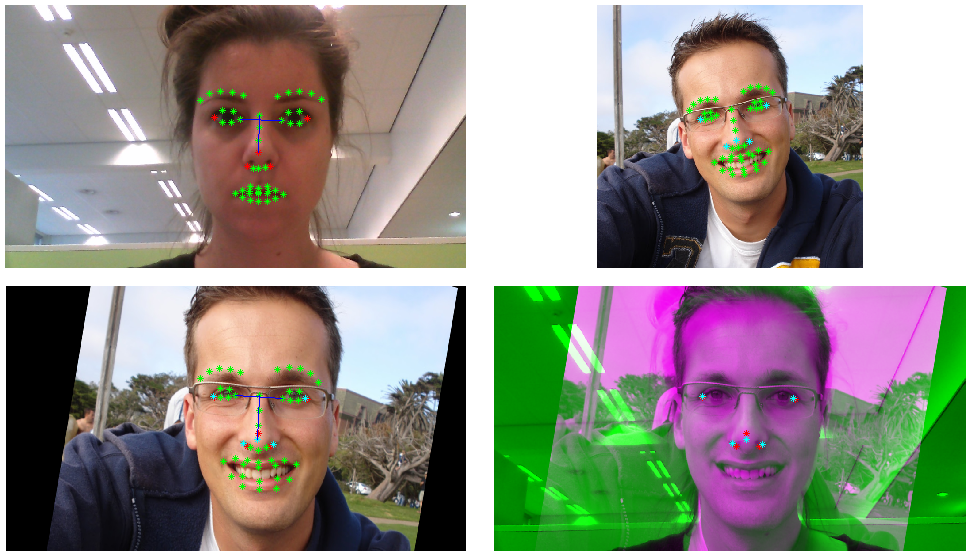
\includegraphics[width=0.5\textwidth]{./ratio.png}
	\caption{Normalized face and ratio}
	\label{fig:ratio}
	\end{center}
\end{figure}

\subsubsection{Normalizing the faces}


\subsubsection{Feature Extraction}


\subsubsection{Classification}


\subsubsection{Decision model}


%------------------------------------------------------------------------------

\section{Experiments}



%------------------------------------------------------------------------------

\section{Results}



%------------------------------------------------------------------------------

\section{Future Works}

\todo[inline]{Add references}

\bibliographystyle{plain}
\bibliography{vision}

\end{document}
